\section{Joc de proves}

Per tal de provar la pràctica s'han realitzat una sèrie de jocs de proves
descrits a continuació. Per cada un d'ells s'ha generat un mapa amb el
\emph{Mapper3Basic} i es poden trobar a la carpeta \emph{maps}.

Al \texttt{Makefile} es troben totes les opcions comentades a l'apartat \emph{sim}, així doncs
es descomenta la desitjada i es comenta la que està per defecte. A continuació
es canvia el codi font
de \texttt{rainer.cpp} comentant el cleanArea i descomentant l'opció desitjada.
Un cop fet això amb un \emph{make} és compila el codi i amb el \emph{make sim}
s'executa el simulador.

El primer test és simple, \textbf{passar per quatre punts sense cap obstacle}. Amb aquest simplement es comprova que es calculi
bé el vector d'atracció. També es pot observar si el \emph{heading} es fa de
manera adequada. Per fer aquesta execució no s'empre cap mapa.

\begin{figure}[H]
\begin{center}\label{4punts}
 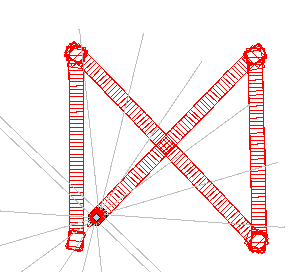
\includegraphics[width=0.5\textwidth]{diagrames/figures/4punts.png}
 % ordreRotacions.png: 1286x768 pixel, 150dpi, 21.77x13.00 cm, bb=0 0 617 369
\end{center}
  \caption{Quatre puts sense obstacle}
\end{figure}

En segon lloc tenim \textbf{passar per quatre punts però amb un obstacle}
enmig. En aquest es veu si l'esquiva d'obstacles es fa bé. A més l'obstacle està
co\lgem ocat de tal manera que el robot es troba impactant una línia de 45 graus
amb el punt destí a la perpendicular, de tal manera que seria una situació
delicada on quedar-se estancat. Per fer aquesta execució s'empra el mapa
\emph{obstacleInclinat}.

\begin{figure}[H]
\begin{center}\label{4puntsObs}
 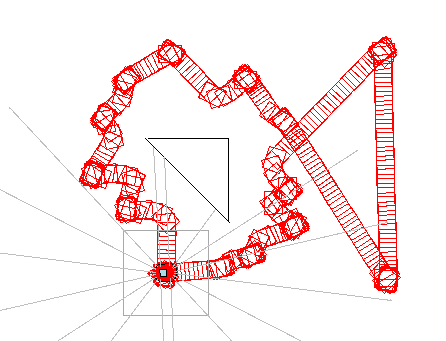
\includegraphics[width=0.5\textwidth]{diagrames/figures/4puntsObs.png}
 % ordreRotacions.png: 1286x768 pixel, 150dpi, 21.77x13.00 cm, bb=0 0 617 369
\end{center}
  \caption{Quatre puts sense obstacle}
\end{figure}

A continuació trobam el mateix \textbf{obstacle} però aquest cop \textbf{situat sobre el punt de destí}, en aquest cas
el robot ha de detectar que no pot arribar-hi ja que l'obstacle i el punt de
destí estan per davall d'un cert llindar. Fins que no s'assoleix aquest llindar
es veu com el robot intenta fer aproximacions al punt desde diferents
direccions. En aquest test empram el mapa \emph{obstacleApunt}.

\begin{figure}[H]
\begin{center}\label{obsapunt}
 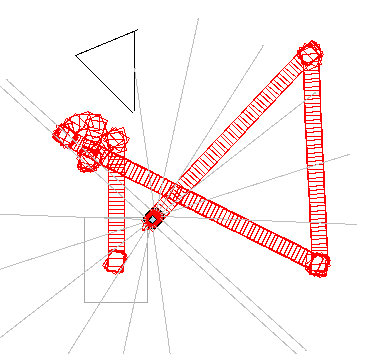
\includegraphics[width=0.5\textwidth]{diagrames/figures/obsapunt.png}
 % ordreRotacions.png: 1286x768 pixel, 150dpi, 21.77x13.00 cm, bb=0 0 617 369
\end{center}
  \caption{Quatre puts sense obstacle}
\end{figure}

Per tal de provar el \textbf{vagar} tenim un mapa tancat amb diversos obstacles
on el robot va rebotant.
Pot arribar un punt en que el robot entri en un cicle ja que els angles de rebot
poden fer que així coincideixi. El que no es permet es que el robot toqui un
obstacle o es quedi immòbil sols girant sobre ell mateix sense ser capaç de
emprendre la ruta cap a una altra banda.

\begin{figure}[H]
\begin{center}\label{vagant}
 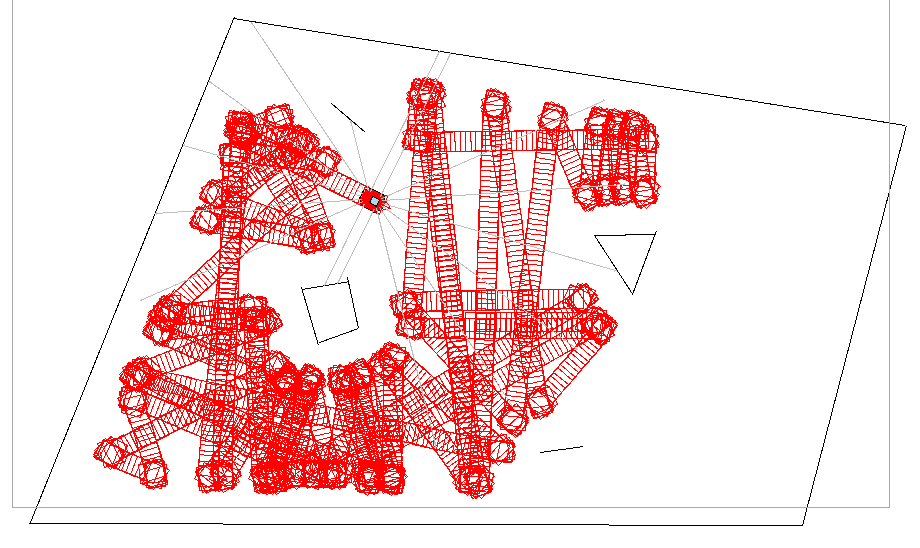
\includegraphics[width=0.5\textwidth]{diagrames/figures/vagant.png}
 % ordreRotacions.png: 1286x768 pixel, 150dpi, 21.77x13.00 cm, bb=0 0 617 369
\end{center}
  \caption{Quatre puts sense obstacle}
\end{figure}

A continuació tenim les proves de la \textbf{neteja de zona}, la primera \textbf{sense obstacles} per veure el recorregut.

\begin{figure}[H]
\begin{center}\label{neteja}
 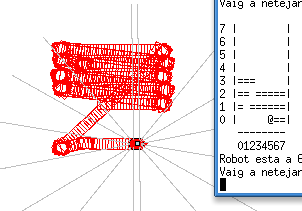
\includegraphics[width=0.5\textwidth]{diagrames/figures/netNoObs.png}
 % ordreRotacions.png: 1286x768 pixel, 150dpi, 21.77x13.00 cm, bb=0 0 617 369
\end{center}
  \caption{Quatre puts sense obstacle}
\end{figure}

I finalment la \textbf{neteja amb obstacles} on el robot els esquiva (i marca terreny durant aquesta esquiva)
i com finalment torna a les zones d'obstacle per comprovar que no fos un
obstacle mòbil i ara si que pot netejar la zona. En aquest últim no podem
simular obstacles mòbils però si veure com torna a intentar anar a la zona
obstaculitzada.

\begin{figure}[H]
\begin{center}\label{netejaobs}
 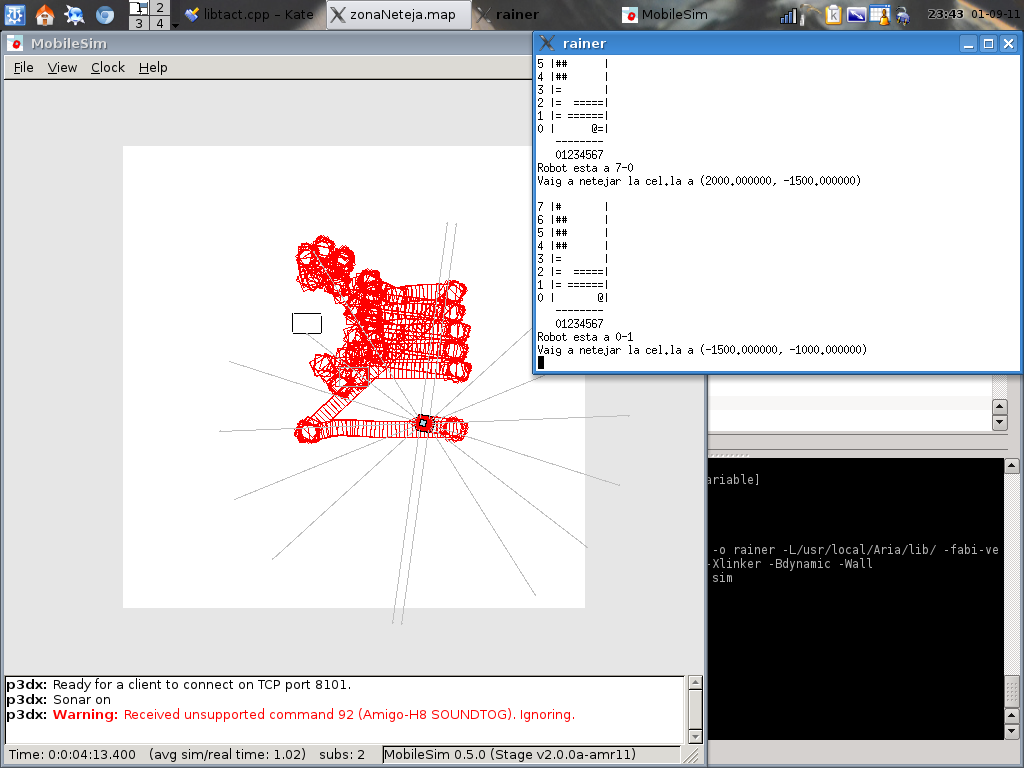
\includegraphics[width=0.5\textwidth]{diagrames/figures/netejant.png}
 % ordreRotacions.png: 1286x768 pixel, 150dpi, 21.77x13.00 cm, bb=0 0 617 369
\end{center}
  \caption{Primera passada de la neteja}
\end{figure}

\begin{figure}[H]
\begin{center}\label{figescenari}
 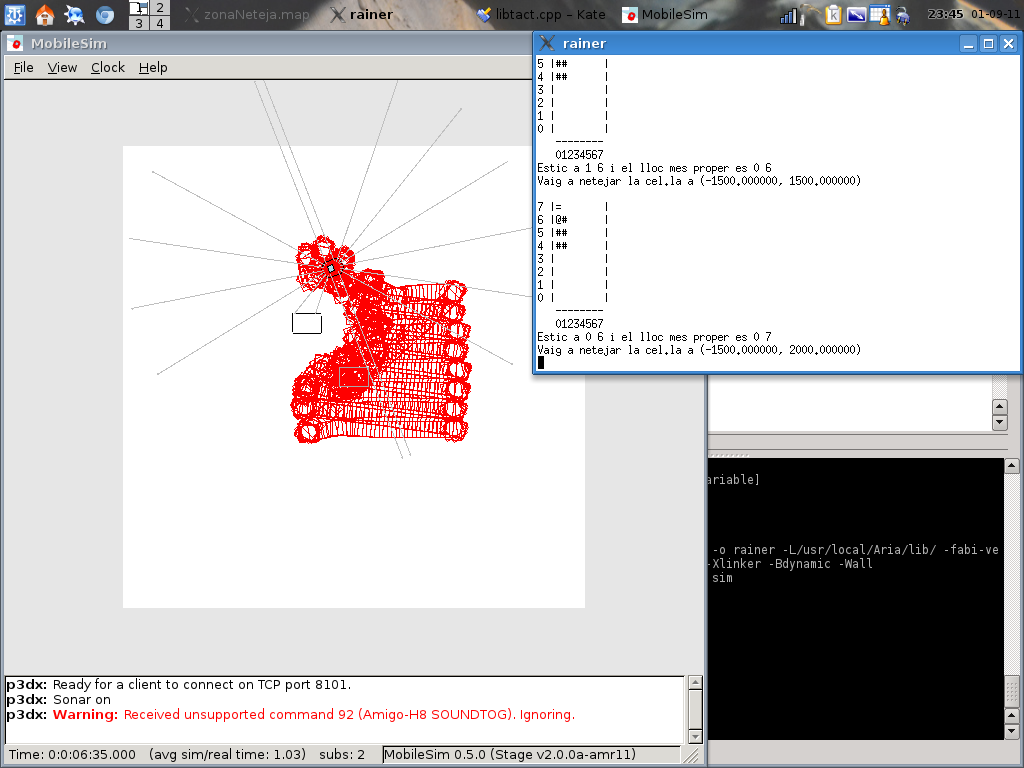
\includegraphics[width=0.5\textwidth]{diagrames/figures/netejant-aobstacles.png}
 % ordreRotacions.png: 1286x768 pixel, 150dpi, 21.77x13.00 cm, bb=0 0 617 369
\end{center}
  \caption{Segona passada de la neteja anant als punts detectats com obstacle}
\end{figure}

